% Version: $Revision$

\section{ANT}

What is ANT? This is how the ANT homepage (\verb=http://ant.apache.org/=) defines its tool:\\

\noindent \emph{Apache Ant is a Java-based build tool. In theory, it is kind of like Make, but without Make's wrinkles.}

\subsection{Basics}

\begin{itemize}
\item the ANT build file is based on XML
\item the usual name for the build file is:
\end{itemize}

\verb=  build.xml=

\begin{itemize}
\item invocation---the usual build file needs not be specified explicitly, if it's in the current directory; if not target is specified, the default one is used
\end{itemize}

\verb=  ant [-f <build-file>] [<target>]=

\begin{itemize}
\item displaying all the available targets of a build file
\end{itemize}

\verb=  ant [-f <build-file>] -projecthelp=

\subsection{Weka and ANT}

\begin{itemize}
\item a build file for Weka is available from subversion
\item some targets of interest
  \begin{itemize}
  \item \verb=clean=--Removes the build, dist and reports directories; also any class files in the source tree
  \item \verb=compile=--Compile weka and deposit class files in\\ \verb=${path_modifier}/build/classes=
  \item \verb=docs=--Make javadocs into \verb=${path_modifier}/doc=
  \item \verb=exejar=--Create an executable jar file in \verb=${path_modifier}/dist=
  \end{itemize}
\end{itemize}

\subsection{Links}
\begin{itemize}
\item ANT homepage: \verb=http://ant.apache.org/=
\item XML: \verb=http://www.w3.org/XML/=
\end{itemize}

% $http://weka.sourceforge.net/wekadoc/index.php/en:ANT_(3.5.6)$

\section{CLASSPATH}
\label{CLASSPATH}
The CLASSPATH environment variable tells Java where to look for
classes. Since Java does the search in a first-come-first-serve kind
of manner, you'll have to take care where and what to put in your
CLASSPATH. I, personally, never use the environment variable, since
I'm working often on a project in different versions in parallel. The
CLASSPATH would just mess up things, if you're not careful (or just
forget to remove an entry). ANT (\verb=http://ant.apache.org/=) offers
a nice way for building (and separating source code and class files)
Java projects. But still, if you're only working on totally separate
projects, it might be easiest for you to use the environment variable.

\subsection{Setting the CLASSPATH} 
In the following we add the \verb=mysql-connector-java-3.1.8-bin.jar=
to our \verb=CLASSPATH= variable (this works for any other jar archive) to make it possible to
access MySQL databases via JDBC.

\subsubsection*{Win32 (2k and XP)}
We assume that the \verb=mysql-connector-java-3.1.8-bin.jar= archive is located in the following directory:\\

\verb=C:\Program Files\Weka-3-5=\\

\noindent In the \emph{Control Panel} click on \emph{System} (or right click on
\emph{My Computer} and select \emph{Properties}) and then go to the
\emph{Avanced} tab. There you'll find a button called \emph{Environment
Variables}, click it. Depending on, whether you're the only person
using this computer or it's a lab computer shared by many, you can
either create a new system-wide (you're the only user) environment
variable or a user dependent one (recommended for multi-user
machines). Enter the following name for the variable.\\

\verb=CLASSPATH=\\

\noindent and add this value\\

\verb=C:\Program Files\Weka-3-5\mysql-connector-java-3.1.8-bin.jar=\\

\noindent If you want to add additional jars, you'll have to separate them with the path separator, the semicolon ; (no spaces!). 

\subsubsection*{Unix/Linux}

We make the assumption that the mysql jar is located in the following directory:\\

\verb=/home/johndoe/jars/=\\

\noindent Open a shell and execute the following command, depending on the shell you're using:

\begin{itemize}
\item bash
\end{itemize}

\verb_export CLASSPATH=$CLASSPATH:/home/johndoe/jars/mysql-connector-java-3.1.8-bin.jar_

\begin{itemize}
\item c shell
\end{itemize}

\verb_setenv CLASSPATH $CLASSPATH:/home/johndoe/jars/mysql-connector-java-3.1.8-bin.jar_

\subsubsection*{Cygwin}

The process is like with Unix/Linux systems, but since the host system
is Win32 and therefore the Java installation also a Win32 application,
you'll have to use the semicolon ; as separator for several jars.

\subsection{RunWeka.bat}
\label{RunWeka.ini}

From version 3.5.4, Weka is launched differently under Win32. The
simple batch file got replaced by a central launcher class
(\verb_= RunWeka.class_) in combination with an INI-file
 (\verb_= RunWeka.ini_). The \verb=RunWeka.bat= only calls this
 launcher class now with the appropriate parameters. With this
 launcher approach it is possible to define different launch
 scenarios, but with the advantage of having placeholders, e.g., for
 the max heap size, which enables one to change the memory for all
 setups easily.

The key of a command in the INI-file is prefixed with \verb=cmd_=, all
other keys are considered placeholders:\\

\verb^cmd_blah=java ...    ^ \emph{command \textbf{blah}}

\verb^bloerk= ...   ^ \emph{placeholder \textbf{bloerk}}\\

\noindent A placeholder is surrounded in a command with \#:\\

\verb^cmd_blah=java #bloerk#^\\

\noindent \textbf{Note:} The key \emph{wekajar} is determined by the
-w parameter with which the launcher class is called.\\

\noindent By default, the following commands are predefined:

\begin{itemize}
\item default\\ The default Weka start, without a terminal window.
\item console\\ For debugging purposes. Useful as Weka gets started from a terminal window.
\item explorer\\ The command that's executed if one double-clicks on an ARFF or XRFF file.
\end{itemize}

\noindent In order to change the \textbf{maximum heap size} for all those commands, one only has
to modify the \textbf{maxheap} placeholder.\\

\noindent For more information check out the comments in the INI-file.

\subsection{java -jar}

When you're using the Java interpreter with the \textbf{-jar} option,
be aware of the fact that it \textbf{overwrites} your \verb=CLASSPATH=
and not \textbf{augments it}. Out of convenience, people often only
use the \textbf{-jar} option to skip the declaration of the main class to
start. But as soon as you need more jars, e.g., for database access,
you need to use the \textbf{-classpath} option and specify the main class.\\

\noindent Here's once again how you start the Weka Main-GUI \textbf{with} your current \verb=CLASSPATH= variable (and 128MB for the JVM):

\begin{itemize}
\item Linux\\ \verb=java -Xmx128m -classpath $CLASSPATH:weka.jar weka.gui.Main=
\item Win32\\ \verb=java -Xmx128m -classpath "%CLASSPATH%;weka.jar" weka.gui.Main=
\end{itemize}

%$http://weka.sourceforge.net/wekadoc/index.php/en:CLASSPATH_(3.5.6)$

\section{Subversion}

\subsection{General}
The Weka \textit{Subversion} repository is accessible and browseable via the following URL:\\

\verb=https://svn.scms.waikato.ac.nz/svn/weka/=\\

\noindent A Subversion repository has usually the following layout:

\begin{verbatim}
root
 |
 +- trunk
 |
 +- tags
 |
 +- branches
\end{verbatim}

\noindent Where \textit{trunk} contains the \textit{main trunk} of the
development, \textit{tags} snapshots in time of the repository (e.g.,
when a new version got released) and \textit{branches} development branches
that forked off the main trunk at some stage (e.g., legacy versions
that still get bugfixed).

\subsection{Source code}
The latest version of the Weka source code can be obtained with this URL:\\

\verb=https://svn.scms.waikato.ac.nz/svn/weka/trunk/weka=\\

\noindent If you want to obtain the source code of the book version, use this URL:\\

\verb=https://svn.scms.waikato.ac.nz/svn/weka/branches/book2ndEd-branch/weka=\\

\subsection{JUnit}
The latest version of Weka's JUnit tests can be obtained with this URL:\\

\verb=https://svn.scms.waikato.ac.nz/svn/weka/trunk/tests=

\noindent And if you want to obtain the JUnit tests of the book version, use this URL:\\

\verb=https://svn.scms.waikato.ac.nz/svn/weka/branches/book2ndEd-branch/tests=

\subsection{Specific version}
Whenever a release of Weka is generated, the repository gets \textit{tagged}

\begin{itemize}
\item \verb=dev-X-Y-Z=\\the tag for a release of the developer version, e.g., \textit{dev-3.5.8} for Weka 3.5.8\\
\verb=https://svn.scms.waikato.ac.nz/svn/weka/tags/dev-3-5-8=
\item \verb=stable-X-Y-Z=\\ the tag for a release of the book version, e.g., \textit{stable-3-4-13} for Weka 3.4.13\\
\verb=https://svn.scms.waikato.ac.nz/svn/weka/tags/stable-3-4-13=
\end{itemize}

\subsection{Clients}
\subsubsection*{Commandline}
Modern Linux distributions already come with Subversion either
pre-installed or easily installed via the package manager of the
distribution. If that shouldn't be case, or if you are using Windows,
you have to download the appropriate client from the Subversion
homepage (\verb=http://subversion.tigris.org/=).

\noindent A checkout of the current developer version of Weka looks like this:\\

\verb=svn co https://svn.scms.waikato.ac.nz/svn/weka/trunk/weka=\\

\subsubsection*{SmartSVN}
SmartSVN (\verb=http://smartsvn.com/=) is a Java-based, graphical,
cross-platform client for Subversion. Though it is not
open-source/free software, the \textit{foundation} version is for free.

\subsubsection*{TortoiseSVN}
Under Windows, TortoiseCVS was a CVS client, neatly integrated into
the Windows Explorer. TortoiseSVN
(\verb=http://tortoisesvn.tigris.org/=) is the equivalent for
Subversion.


\section{GenericObjectEditor}

\subsection{Introduction}
As of version 3.4.4 it is possible for Weka to dynamically discover
classes at runtime (rather than using only those specified in the
\verb=GenericObjectEditor.props= (GOE) file). In version 3.5.8 and higher
this facility is not enabled by default as it is slower than the props file
approach, and, furthermore, does not function in environments that do
not have a CLASSPATH (e.g. application servers).

If you wish to use dynamic class discovery, the relevant file to edit
is\\ \verb=GenericPropertiesCreator.props= (GPC, located in
weka.gui). All that is required is to change the \verb=UseDynamic=
property in this file from \verb=false= to \verb=true=.

If dynamic class discovery is too slow, e.g., due to an enormous CLASSPATH, you can
generate a new \verb=GenericObjectEditor.props= file and then turn dynamic
class discovery off again. Just follow these steps:

\begin{itemize}
\item generate a new \verb=GenericObjectEditor.props= file, based on your current setup (assuming the weka classes are in your CLASSPATH and you're currently just above the root package):\\ \\
\verb=java weka.gui.GenericPropertiesCreator \= \\
\verb=weka/gui/GenericPropertiesCreator.props \= \\
\verb=$HOME/GenericObjectEditor.props=\\ \\
this will generate a new props file in your home directory (Windows users have to replace the \verb=$HOME= 
\verb=with %USERPROFILE%=).

\item edit the \verb=GenericPropertiesCreator.props= file and set \verb=UseDynamic= to \verb=false=
\end{itemize}

\noindent Like with the GOE file the GPC can be either modified in its original
position (inside the source tree), or you can place a copy of it in
your home directory and modify this one - which makes installing WEKA
updates easier, by just replacing the weka.jar.

A limitation of the GOE was so far that additional classifiers,
filters etc. had to fit into the same package structure as the already
existing ones, i.e. all had to be located below weka. WEKA can now
display multiple class hierarchies in the GUI, which makes adding new
functionality quite easy as we will see later in an example (it is not
restricted to classifiers only, but also works with all the other
entries in the GPC file).

\subsection{File Structure}
The structure of the GOE is a key-value-pair, separated by an
equals-sign. The value is a comma separated list of classes that are
all derived from the superclass/superinterface \textit{key}. The GPC is
slightly different, instead of declaring all the classes/interfaces
one need only to specify all the packages descendants are located in
(only non-abstract ones are then listed). E.g., the
\verb=weka.classifiers.Classifier= entry in the GOE file looks like this:

\begin{verbatim}
weka.classifiers.Classifier=\
 weka.classifiers.bayes.AODE,\
 weka.classifiers.bayes.BayesNet,\
 weka.classifiers.bayes.ComplementNaiveBayes,\
 weka.classifiers.bayes.NaiveBayes,\
 weka.classifiers.bayes.NaiveBayesMultinomial,\
 weka.classifiers.bayes.NaiveBayesSimple,\
 weka.classifiers.bayes.NaiveBayesUpdateable,\
 weka.classifiers.functions.LeastMedSq,\
 weka.classifiers.functions.LinearRegression,\
 weka.classifiers.functions.Logistic,\
 ...
\end{verbatim}

\noindent The entry producing the same output for the classifiers in the GPC looks like this (7 lines instead of over 70):

\begin{verbatim}
weka.classifiers.Classifier=\
 weka.classifiers.bayes,\
 weka.classifiers.functions,\
 weka.classifiers.lazy,\
 weka.classifiers.meta,\
 weka.classifiers.trees,\
 weka.classifiers.rules
\end{verbatim}

\subsection{Exclusion}
It may not always be desired to list all the classes that can be found
along the \verb=CLASSPATH=. Sometimes, classes cannot be declared \verb=abstract=
but still shouldn't be listed in the GOE. For that reason one can list
classes, interfaces, superclasses for certain packages to be excluded
from display. This exclusion is done with the following file:\\

\verb=weka/gui/GenericPropertiesCreator.excludes=\\

\noindent The format of this properties file is fairly simple:\\

\verb^<key>=<prefix>:<class>[,<prefix>:<class>]^\\

\noindent Where the \verb=<key>= corresponds to a key in the
\verb=GenericPropertiesCreator.props= file and the \verb=<prefix>= can
be one of the following:

\begin{itemize}
\item \textbf{S} -- \textit{Superclass}\\
  any class derived from this will be excluded
\item \textbf{I} -- \textit{Interface}\\
  any class implementing this interface will be excluded
\item \textbf{C} -- \textit{Class}\\
  exactly this class will be excluded
\end{itemize}

\noindent Here are a few examples:

\begin{verbatim}
# exclude all ResultListeners that also implement the ResultProducer interface
# (all ResultProducers do that!)
weka.experiment.ResultListener=\
  I:weka.experiment.ResultProducer

# exclude J48 and all SingleClassifierEnhancers
weka.classifiers.Classifier=\
  C:weka.classifiers.trees.J48,\
  S:weka.classifiers.SingleClassifierEnhancer
\end{verbatim}

\subsection{Class Discovery}
Unlike the \verb=Class.forName(String)= method that grabs the first class it
can find in the \verb=CLASSPATH=, and therefore fixes the location of the
package it found the class in, the dynamic discovery examines the
complete \verb=CLASSPATH= you're starting the Java Virtual Machine (= JVM)
with. This means that you can have several parallel directories with
the same WEKA package structure, e.g. the standard release of WEKA in
one directory (\verb=/distribution/weka.jar=) and another one with your own
classes (\verb=/development/weka/...=), and display all of the classifiers in
the GUI. In case of a name conflict, i.e. two directories contain the
same class, the first one that can be found is used. In a nutshell,
your java call of the Experimenter can look like this:\\

\verb=java -classpath "/development:/distribution/weka.jar" weka.gui.experiment.Experimenter=\\

\noindent \textit{Note: Windows users have to replace the ``:'' with ``;''}\\

\subsection{Multiple Class Hierarchies}
In case you're developing your own framework, but still want to use
your classifiers within WEKA that wasn't possible so far. With the
release 3.4.4 it is possible to have multiple class hierarchies being
displayed in the GUI. If you've developed a modified version of NaiveBayes,
let's call it \textit{DummyBayes} and it's located in the package\verb= dummy.classifiers=
then you'll have to add this package to the classifiers list in the
GPC file like this:

\begin{verbatim}
weka.classifiers.Classifier=\
 weka.classifiers.bayes,\
 weka.classifiers.functions,\
 weka.classifiers.lazy,\
 weka.classifiers.meta,\
 weka.classifiers.trees,\
 weka.classifiers.rules,\
 dummy.classifiers
\end{verbatim}

\noindent Your java call for the Experimenter might look like this:

\verb=java -classpath "weka.jar:dummy.jar" weka.gui.experiment.Experimenter=\\

\noindent Starting up the GUI you'll now have another root node in the
tree view of the classifiers, called \textit{root}, and below it the weka and
the \textit{dummy} package hierarchy as you can see here:

\begin{center}
\epsfig{file=images/technical/En-goe-353.eps,height=7cm}
\end{center}

\subsection{Capabilities}
Version \textbf{3.5.3} of Weka introduced the notion of
\textit{Capabilities}. Capabilities basically list what kind of data a
certain object can handle, e.g., one classifier can handle numeric
classes, but another cannot. In case a class supports capabilities the
additional buttons \textbf{Filter...} and \textbf{Remove filter} will
be available in the GOE. The Filter... button pops up a dialog which
lists all available Capabilities:

\begin{center}
\epsfig{file=images/technical/En-goe-filter-353.eps,height=7cm}
\end{center}

\noindent One can then choose those capabilities an object, e.g., a
classifier, should have. If one is looking for classification problem,
then the \textit{Nominal} class Capability can be selected. On the other hand,
if one needs a regression scheme, then the Capability \textit{Numeric} class
can be selected. This filtering mechanism makes the search for an
appropriate learning scheme easier. After applying that filter, the
tree with the objects will be displayed again and lists all objects
that can handle all the selected Capabilities black, the ones that
cannot grey and the ones that might be able to handle them blue (e.g.,
meta classifiers which depend on their base classifier(s)).

\section{Properties}
A properties file is a simple text file with this structure:\\

\verb^<key>=<value>^\\

\noindent Comments start with the hash sign \#.\\

\noindent To make a rather long property line more readable, one can
use a backslash to continue on the next line. The Filter property,
e.g., looks like this:

\begin{verbatim}
weka.filters.Filter= \
 weka.filters.supervised.attribute, \
 weka.filters.supervised.instance, \
 weka.filters.unsupervised.attribute, \
 weka.filters.unsupervised.instance
\end{verbatim}

\subsection{Precedence}
The Weka property files (extension .props) are searched for in the following order:

\begin{itemize}
\item current directory
\item the user's home directory (*nix \verb=$HOME=, Windows \verb=%USERPROFILE%=)
\item the class path (normally the weka.jar file) 
\end{itemize}

\noindent If Weka encounters those files it only supplements the
properties, never overrides them. In other words, a property in the
property file of the current directory has a higher precedence than
the one in the user's home directory.\\

\noindent Note: Under Cywgin (http://cygwin.com/), the home directory
is still the Windows one, since the java installation will be still
one for Windows.

\subsection{Examples}

\begin{itemize}
\item weka/gui/LookAndFeel.props
\item weka/gui/GenericPropertiesCreator.props
\item weka/gui/beans/Beans.props
\end{itemize}


\section{XML}
Weka now supports XML (\verb=http://www.w3c.org/XML/=) (eXtensible
Markup Language) in several places.

\subsection{Command Line}
\label{xml_command_line}
WEKA now allows Classifiers and Experiments to be started using an
\verb=-xml= option followed by a filename to retrieve the command line
options from the XML file instead of the command line.

For such simple classifiers like e.g. J48 this looks like overkill,
but as soon as one uses Meta-Classifiers or Meta-Meta-Classifiers the
handling gets tricky and one spends a lot of time looking for missing
quotes. With the hierarchical structure of XML files it is simple to
plug in other classifiers by just exchanging tags.

The DTD for the XML options is quite simple:

\begin{verbatim}
<!DOCTYPE options
[
   <!ELEMENT options (option)*>
   <!ATTLIST options type CDATA "classifier">
   <!ATTLIST options value CDATA "">
   <!ELEMENT option (#PCDATA | options)*>
   <!ATTLIST option name CDATA #REQUIRED>
   <!ATTLIST option type (flag | single | hyphens | quotes) "single">
]
>
\end{verbatim}

\noindent The type attribute of the option tag needs some
explanations. There are currently four different types of options in
WEKA:

\begin{itemize}
\item \textbf{flag}\\
The simplest option that takes no arguments, like e.g. the -V flag for inversing an selection.\\\\
\verb^<option name="V" type="flag"/>^
\item \textbf{single}\\ 
The option takes exactly one parameter,
  directly following after the option, e.g., for specifying the
  trainings file with \verb=-t somefile.arff=. Here the parameter value is
  just put between the opening and closing tag. Since single is the
  default value for the type tag we don't need to specify it
  explicitly.\\\\
\verb^<option name="t">somefile.arff</option>^
\item \textbf{hyphens}\\
Meta-Classifiers like \verb=AdaBoostM1= take another classifier as option
with the \verb=-W= option, where the options for the base classifier follow
after the \verb=--=. And here it is where the fun starts: where to put
parameters for the base classifier if the Meta-Classifier itself is a
base classifier for another Meta-Classifier?\\

E.g., does \verb=-W weka.classifiers.trees.J48 -- -C 0.001= become this:
\begin{verbatim}
<option name="W" type="hyphens">
   <options type="classifier" value="weka.classifiers.trees.J48">
      <option name="C">0.001</option>
   </options>
</option>
\end{verbatim}

\noindent Internally, all the options enclosed by the \verb=options= tag are
pushed to the end after the \verb=--= if one transforms the XML into a
command line string.

\item \textbf{quotes}\\
A Meta-Classifier like \verb=Stacking= can take several \verb=-B= options, where
each single one encloses other options in quotes (this itself can
contain a Meta-Classifier!). From \verb=-B ``weka.classifiers.trees.J48''= we
then get this XML:\\
\begin{verbatim}
<option name="B" type="quotes">
   <options type="classifier" value="weka.classifiers.trees.J48"/>
</option>
\end{verbatim}

\noindent With the XML representation one doesn't have to worry
anymore about the level of quotes one is using and therefore doesn't
have to care about the correct escaping (i.e. \verb=`` ... \" ... \" ...''=)
since this is done automatically.

And if we now put all together we can transform this more complicated
command line (\verb=java= and the \verb=CLASSPATH= omitted):

\begin{verbatim}
<options type="class" value="weka.classifiers.meta.Stacking">
   <option name="B" type="quotes">
      <options type="classifier" value="weka.classifiers.meta.AdaBoostM1">
         <option name="W" type="hyphens">
            <options type="classifier" value="weka.classifiers.trees.J48">
               <option name="C">0.001</option>
            </options>
         </option>
      </options>
   </option>
   
   <option name="B" type="quotes">
      <options type="classifier" value="weka.classifiers.meta.Bagging">
         <option name="W" type="hyphens">
            <options type="classifier" value="weka.classifiers.meta.AdaBoostM1">
               <option name="W" type="hyphens">
                  <options type="classifier" value="weka.classifiers.trees.J48"/>
               </option>
            </options>
         </option>
      </options>
   </option>

   <option name="B" type="quotes">
      <options type="classifier" value="weka.classifiers.meta.Stacking">
         <option name="B" type="quotes">
            <options type="classifier" value="weka.classifiers.trees.J48"/>
         </option>
      </options>
   </option>

   <option name="t">test/datasets/hepatitis.arff</option>
</options>
\end{verbatim}
\end{itemize}

\noindent \textbf{Note}: The \verb=type= and \verb=value= attribute of the outermost
\verb=option=s tag is not used while reading the parameters. It is merely for
documentation purposes, so that one knows which class was actually
started from the command line.\\

\noindent \textbf{Responsible Class(es)}:

\begin{verbatim}
weka.core.xml.XMLOptions
\end{verbatim}

\subsection{Serialization of Experiments}
It is now possible to serialize the Experiments from the WEKA
Experimenter not only in the proprietary binary format Java offers
with serialization (with this you run into problems trying to read old
experiments with a newer WEKA version, due to different SerialUIDs),
but also in XML. There are currently two different ways to do this:

\begin{itemize}
\item \textbf{built-in}\\
The built-in serialization captures only the necessary informations of
an experiment and doesn't serialize anything else. It's sole purpose
is to save the setup of a specific experiment and can therefore not
store any built models. Thanks to this limitation we'll never run into
problems with mismatching SerialUIDs.

This kind of serialization is always available and can be selected via
a Filter (*.xml) in the Save/Open-Dialog of the Experimenter.

The DTD is very simple and looks like this (for version 3.4.5): 

\begin{verbatim}
<!DOCTYPE object[
   <!ELEMENT object (#PCDATA | object)*>
   <!ATTLIST object name      CDATA #REQUIRED>
   <!ATTLIST object class     CDATA #REQUIRED>
   <!ATTLIST object primitive CDATA "no">
   <!ATTLIST object array     CDATA "no">   
   <!ATTLIST object null      CDATA "no">   
   <!ATTLIST object version   CDATA "3.4.5">
]>
\end{verbatim}

\noindent Prior to versions 3.4.5 and 3.5.0 it looked like this: 

\begin{verbatim}
<!DOCTYPE object
[
   <!ELEMENT object (#PCDATA | object)*>
   <!ATTLIST object name      CDATA #REQUIRED>
   <!ATTLIST object class     CDATA #REQUIRED>
   <!ATTLIST object primitive CDATA "yes">
   <!ATTLIST object array     CDATA "no">
]
>
\end{verbatim}

\noindent \textbf{Responsible Class(es)}:\\

\verb=weka.experiment.xml.XMLExperiment=\\

\noindent \textbf{for general Serialization}:

\begin{verbatim}
weka.core.xml.XMLSerialization
weka.core.xml.XMLBasicSerialization 
\end{verbatim}

\item \textbf{KOML} (\verb=http://koala.ilog.fr/XML/serialization/=)\\
The Koala Object Markup Language (KOML) is published under the LGPL
(http://www.gnu.org/copyleft/lgpl.html) and is an alternative way of
serializing and derserializing Java Objects in an XML file. Like the
normal serialization it serializes everything into XML via an
ObjectOutputStream, including the SerialUID of each class. Even though
we have the same problems with mismatching SerialUIDs it is at least
possible edit the XML files by hand and replace the offending IDs with
the new ones.

In order to use KOML one only has to assure that the KOML classes are
in the CLASSPATH with which the Experimenter is launched. As soon as
KOML is present another Filter (\verb=*.koml=) will show up in the
Save/Open-Dialog.

The DTD for KOML can be found at \verb=http://koala.ilog.fr/XML/koml12.dtd=\\

\noindent \textbf{Responsible Class(es)}:\\

\verb=weka.core.xml.KOML=\\
\end{itemize}

\noindent The experiment class can of course read those XML files if passed as
input or output file (see options of \verb=weka.experiment.Experiment= and
\verb=weka.experiment.RemoteExperiment=

\subsection{Serialization of Classifiers}
The options for models of a classifier, \verb=-l= for the input model and \verb=-d=
for the output model, now also supports XML serialized files. Here we
have to differentiate between two different formats:

\begin{itemize}
\item \textbf{built-in}\\
The built-in serialization captures only the options of a classifier
but not the built model. With the \verb=-l= one still has to provide a
training file, since we only retrieve the options from the XML
file. It is possible to add more options on the command line, but it
is no check performed whether they collide with the ones stored in the
XML file.

The file is expected to end with \verb=.xml=.

\item \textbf{KOML}\\
Since the KOML serialization captures everything of a Java Object we
can use it just like the normal Java serialization.

The file is expected to end with \verb=.koml=.
\end{itemize}

\noindent The \textbf{built-in} serialization can be used in the
\textbf{Experimenter} for loading/saving options from algorithms that
have been added to a Simple Experiment. Unfortunately it is not
possible to create such a hierarchical structure like mentioned in
Section~\ref{xml_command_line}. This is because of the loss of
information caused by the \verb=getOptions()= method of classifiers: it
returns only a flat String-Array and not a tree structure.\\

\noindent \textbf{Responsible Class(es)}:

\begin{verbatim}
weka.core.xml.KOML
weka.classifiers.xml.XMLClassifier
\end{verbatim}

\subsection{Bayesian Networks}
The GraphVisualizer (\verb=weka.gui.graphvisualizer.GraphVisualizer=) can
save graphs into the Interchange Format\\
(\verb=http://www-2.cs.cmu.edu/~fgcozman/Research/InterchangeFormat/=) for
Bayesian Networks (BIF). If started from command line with an XML
filename as first parameter and not from the Explorer it can display
the given file directly.

The DTD for BIF is this:

\begin{verbatim}
<!DOCTYPE BIF [
   <!ELEMENT BIF ( NETWORK )*>
         <!ATTLIST BIF VERSION CDATA #REQUIRED>
   <!ELEMENT NETWORK ( NAME, ( PROPERTY | VARIABLE | DEFINITION )* )>
   <!ELEMENT NAME (#PCDATA)>

   <!ELEMENT VARIABLE ( NAME, ( OUTCOME |  PROPERTY )* ) >
         <!ATTLIST VARIABLE TYPE (nature|decision|utility) "nature">
   <!ELEMENT OUTCOME (#PCDATA)>
   <!ELEMENT DEFINITION ( FOR | GIVEN | TABLE | PROPERTY )* >
   <!ELEMENT FOR (#PCDATA)>
   <!ELEMENT GIVEN (#PCDATA)>

   <!ELEMENT TABLE (#PCDATA)>
   <!ELEMENT PROPERTY (#PCDATA)>
]>
\end{verbatim}

\noindent \textbf{Responsible Class(es)}:

\begin{verbatim}
weka.classifiers.bayes.BayesNet#toXMLBIF03()
weka.classifiers.bayes.net.BIFReader
weka.gui.graphvisualizer.BIFParser
\end{verbatim}

\subsection{XRFF files}
With Weka 3.5.4 a new, more feature-rich, XML-based data format got
introduced: \textbf{XRFF}. For more information, please see
Chapter~\ref{xrff}.

%$http://weka.sourceforge.net/wekadoc/index.php/en:XML_(3.5.6)$
